\documentclass[11pt]{article}
\usepackage[margin=1in]{geometry}
\usepackage{lmodern}
\usepackage{setspace}
\usepackage{booktabs}
\usepackage{array}
\usepackage{graphicx}
\usepackage{hyperref}
\usepackage{amsmath}
\usepackage{authblk}
\usepackage[authoryear,round]{natbib}
\usepackage{enumitem}
\usepackage{xcolor}
\usepackage{microtype}
\usepackage{url}
\usepackage[T1]{fontenc}
\usepackage[utf8]{inputenc}
\usepackage{tikz}
\usetikzlibrary{shapes.geometric,arrows.meta,positioning,fit,backgrounds}
\usepackage{fancyhdr}
\onehalfspacing
\setlength{\parindent}{0.4in}
\hypersetup{colorlinks=true,linkcolor=blue,citecolor=blue,urlcolor=blue}

\pagestyle{fancy}
\fancyhf{}
\rhead{\small SAFE-EAR}
\lhead{\small Deterministic Referral Safety over LLM Extraction}
\cfoot{\thepage}
\renewcommand{\headrulewidth}{0.4pt}

\title{A Deterministic, Guideline-Derived Referral-Safety Layer over Open Medical-LLM Extraction for Time-Critical Otologic Symptoms\\[2pt]
\large An Open Benchmark and Reproducible Evaluation (SAFE-EAR)}
\author[1]{Geunsik Lim}
\author[2]{Hyun Jo}
\affil[1]{Sungkyunkwan University, Republic of Korea; \texttt{leemgs@g.skku.edu}}
\affil[2]{Ajou University School of Medicine, Republic of Korea; \texttt{joehyun@ajou.ac.kr}}
\date{}

\begin{document}
\maketitle
\thispagestyle{fancy}

\begin{center}
\small
\begin{tabular}{@{}l p{0.66\textwidth}@{}}
\textbf{Article type:} & Methods / open-benchmark study (safety engineering for clinical AI) \\
\textbf{Target venue:} & Digital-health / medical-informatics journal (e.g., \textit{JAMIA Open}, \textit{npj Digital Medicine}, \textit{JMIR AI}) \\
\textbf{Companion paper:} & The empirical STARS survey study (perceived stress, tinnitus, audiometric thresholds); this paper develops STARS's prospective safety/extraction component \emph{with results} \\
\textbf{Reporting:} & TRIPOD+AI-aligned; open code, benchmark, and metrics \\
\textbf{Data:} & Expert-authored / synthetic only --- \emph{no patient data} \\
\end{tabular}

\vspace{2pt}
{\footnotesize\emph{Note.} This paper reports \textbf{real} results for a deterministic safety layer and a reproducible rule-based extraction baseline on an open benchmark. Evaluation of an actual open medical LLM (e.g., MedGemma) on clinical free text is a prospective step requiring model access and IRB-approved data; the benchmark and metrics are fixed here so that comparison is prespecified.}
\end{center}

\begin{abstract}
\noindent\textbf{Background:} Large language models (LLMs) can extract structured audiology fields from clinical text, but a probabilistic model must never be allowed to suppress referral for a time-critical emergency such as sudden sensorineural hearing loss (SSNHL), whose treatment window is narrow. \textbf{Objective:} To specify and \emph{evaluate} a deterministic, guideline-derived red-flag safety layer that overrides model output, and to release an open benchmark and reproducible evaluation harness. \textbf{Methods:} We derive seven red-flag rules from the SSNHL and tinnitus clinical practice guidelines and evaluate them at two levels on an open benchmark of 41 expert-authored/synthetic cases (20 structured, 21 free-text; no patient data): (i) \emph{rule coverage} on correctly-extracted features, and (ii) \emph{end-to-end}, running free text through an open, deterministic rule-based extraction baseline first. We report red-flag recall (the safety-critical metric) with 95\% Wilson confidence intervals, specificity, over-referral, per-note-category breakdowns, and per-field extraction metrics. \textbf{Results:} On correctly-extracted features the layer achieved complete guideline coverage---sensitivity 100\% (12/12) and specificity 100\% (8/8), i.e., zero over-referral. End-to-end, recall fell to 82\% (9/11; 95\% CI 52--95) and specificity to 90\% (9/10; 95\% CI 60--98): two urgent presentations phrased without canonical keywords were missed and one \emph{resolved historical} SSNHL mention produced a false alarm. The rule-based extraction baseline reached macro-F1 0.87 (precision 0.93, recall 0.84), document-level exact feature match 0.67, an urgency-changing error rate of 14\%, and perfect run-to-run consistency. \textbf{Conclusions:} A deterministic safety layer can \emph{guarantee} that a low model score never suppresses referral and, given correct features, misses no guideline red flag; but end-to-end recall is bounded by extraction, so mandatory clinician verification is load-bearing, not optional. We release the benchmark, rules, extractor, and metrics as a prespecified reference for future open-LLM (e.g., MedGemma) evaluation.
\end{abstract}

\noindent\textbf{Keywords:} clinical NLP; large language models; MedGemma; patient safety; guardrails; sudden sensorineural hearing loss; tinnitus; referral triage; open benchmark; reproducibility.

\section{Introduction}
Sudden sensorineural hearing loss (SSNHL) is an otologic emergency: prompt audiometric confirmation and early corticosteroid therapy---within roughly two weeks---offer the best chance of recovery, and delayed presentation is associated with worse outcomes \citep{chandrasekhar2019ssnhl}. In an era of LLM-assisted clinical documentation and triage, a foreseeable failure mode is that a probabilistic model, extracting or summarizing a patient narrative, assigns a reassuring ``low-risk / likely stress'' interpretation to what is in fact an acute asymmetric loss---and thereby contributes to delay. The motivating companion study (STARS) shows that perceived stress tracks the tinnitus \emph{symptom} more than the audiometric \emph{threshold}; precisely because ``stress-related tinnitus'' is common and usually benign, the dangerous case is the rare acute presentation hiding among many benign ones.

The safe design principle is therefore not a better classifier but a \emph{non-overridable floor}: a deterministic, guideline-derived rule layer that screens for red flags and forces urgent referral regardless of any model score. This paper specifies that layer, and---unlike a design-only proposal---\emph{evaluates} it on an open benchmark, quantifying both its guideline coverage and, honestly, the residual risk introduced when an imperfect extraction step feeds it.

\paragraph{Contributions.}
\begin{enumerate}[leftmargin=1.5em,itemsep=1pt]
\item A deterministic red-flag safety layer derived from the SSNHL and tinnitus clinical practice guidelines \citep{chandrasekhar2019ssnhl,tunkel2014cpg}, which overrides model output and cannot be suppressed by a low predicted risk.
\item An \textbf{open benchmark} (41 expert-authored/synthetic cases; no patient data) and a \textbf{two-level evaluation} that separates \emph{rule coverage} (on correct features) from \emph{end-to-end} performance (on free text), isolating where risk actually arises.
\item \textbf{Real results}: complete rule coverage (100\% recall, 0\% over-referral) but end-to-end recall bounded by extraction (82\%), with a reproducible rule-based extraction baseline (macro-F1 0.87) released as a prespecified reference for future open-LLM (e.g., MedGemma) comparison.
\item Open code, rules, benchmark, and metrics, so the evaluation is reproducible and extensible.
\end{enumerate}

\section{Related Work}
Clinical information extraction with LLMs is advancing rapidly, and open medical models such as MedGemma are positioned as starting points for health-AI development rather than validated devices \citep{medgemma2025blog,medgemma2026docs}. Reporting standards for clinical prediction/AI emphasize prespecified evaluation and transparency \citep{collins2024tripodai}. A recurring theme in safety-critical clinical AI is that probabilistic components should be wrapped in deterministic guardrails for time-critical decisions; our contribution is a concrete, guideline-traceable instance for otology, released \emph{with} an open benchmark and honest end-to-end numbers rather than an asserted target. The clinical endpoints follow the SSNHL and tinnitus guidelines \citep{chandrasekhar2019ssnhl,tunkel2014cpg}. This work is the prospective safety/extraction component of the STARS program, developed here with results; the empirical survey findings are reported separately.

\section{System Design}
\subsection{Architecture: extraction, then a non-overridable safety floor}
The pipeline (Figure~\ref{fig:arch}) is deliberately ordered so the safety layer is last and authoritative: free text is first mapped by a \emph{schema-constrained} extractor to typed fields and boolean red-flag features; the \emph{deterministic} layer then evaluates guideline rules over those features and, if any fires, returns an urgent-referral message that \emph{overrides} any probabilistic output. A low model score can never suppress this message.

\begin{figure}[htbp]
\centering
\resizebox{\textwidth}{!}{%
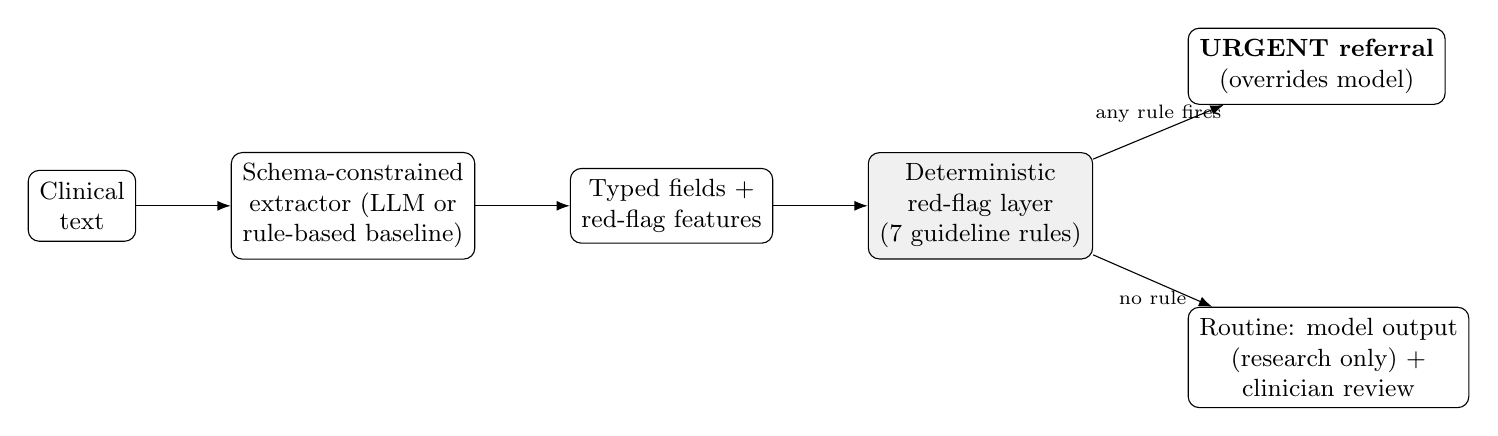
\begin{tikzpicture}[
  node distance=8mm and 12mm, >=Latex,
  box/.style={draw, rounded corners, align=center, inner sep=4pt, font=\small, minimum height=9mm},
  safe/.style={draw, rounded corners, align=center, inner sep=4pt, font=\small, minimum height=9mm, fill=black!6},
]
\node[box] (text) {Clinical\\text};
\node[box, right=of text] (extract) {Schema-constrained\\extractor (LLM or\\rule-based baseline)};
\node[box, right=of extract] (feat) {Typed fields +\\red-flag features};
\node[safe, right=of feat] (safety) {Deterministic\\red-flag layer\\(7 guideline rules)};
\node[box, above right=6mm and 12mm of safety] (urgent) {\textbf{URGENT referral}\\(overrides model)};
\node[box, below right=6mm and 12mm of safety] (routine) {Routine: model output\\(research only) +\\clinician review};
\draw[->] (text) -- (extract);
\draw[->] (extract) -- (feat);
\draw[->] (feat) -- (safety);
\draw[->] (safety) -- node[above,font=\scriptsize]{any rule fires} (urgent);
\draw[->] (safety) -- node[below,font=\scriptsize]{no rule} (routine);
\end{tikzpicture}%
}
\caption{The deterministic red-flag layer is the last, authoritative stage: any guideline red flag forces urgent referral and overrides probabilistic output. The extractor may be an open LLM (e.g., MedGemma) or the reproducible rule-based baseline evaluated here.}
\label{fig:arch}
\end{figure}

\subsection{Guideline-derived red-flag rules}
Seven rules encode time-critical presentations from the SSNHL and tinnitus guidelines \citep{chandrasekhar2019ssnhl,tunkel2014cpg}: (1) sudden hearing loss; (2) rapidly progressive loss; (3) unilateral sudden symptom; (4) acute aural fullness with a sudden drop; (5) single-sided tinnitus \emph{with} audiometric asymmetry (a combined rule); (6) vertigo; and (7) a focal neurologic sign. The decision is a logical OR across rules; combined rules require all their indicators. The rules are intentionally conservative---a missed red flag (a false negative) is the costly error---and deterministic, so their behavior is fully auditable and reproducible.

\subsection{Governance}
The extractor is constrained to a fixed schema with typed fields; free-text generation is disallowed for structured outputs, every field carries a rule-based reliability flag (source-span agreement, \emph{not} the model's token probability), and every field is clinician-verified before entering analysis. The safety layer supplements, never replaces, clinical assessment: a finite-set sensitivity of 1.00 is a target, not a guarantee of zero deployment misses.

\section{Benchmark and Evaluation}
\subsection{Open benchmark (no patient data)}
Because clinical text requires IRB approval and deidentification, the benchmark is entirely expert-authored or synthetic and can be released openly. It contains 41 cases: 20 \emph{structured} cases (12 guideline-urgent, 8 benign) whose gold urgency is assigned a priori from the guidelines \emph{independently} of the rule code, and 21 \emph{free-text} notes (11 urgent, 10 benign) spanning four categories---\emph{typical} (clean phrasing), \emph{negation} (explicit negatives), \emph{colloquial} (lay phrasing), and \emph{ambiguous} (vague onset/laterality)---including cases where an urgent presentation is described \emph{without} canonical keywords. Each case carries laterality/onset/vertigo metadata for subgroup analysis.

\subsection{Two-level evaluation}
We evaluate at two levels. \textbf{Rule coverage} applies the deterministic layer to the correctly-extracted structured features, testing whether the rule set flags every guideline red flag and avoids over-flagging benign presentations. \textbf{End-to-end} runs each free-text note through the schema-constrained rule-based extractor and then the safety layer, so extraction error can propagate. Red-flag recall (sensitivity) is the safety-critical metric; we also report specificity and over-referral, with 95\% Wilson confidence intervals, and per-note-category performance.

\subsection{Reproducible extraction baseline}
The extractor is an open, deterministic rule-based reference (normalized keyword cues with a short negation window). It is not intended to be state-of-the-art; it fixes the harness and gold so that an open medical LLM (e.g., MedGemma) can later be evaluated against an identical, prespecified target. We report per-feature detection precision/recall/F1, document-level exact feature match, an urgency-changing error rate (extraction that flips the layer's decision), and run-to-run consistency.

\section{Results}
\subsection{The deterministic layer: complete coverage, extraction-bounded end-to-end}
On correctly-extracted features the layer flagged every guideline red flag and over-referred none: sensitivity 100\% (12/12) and specificity 100\% (8/8) (Table~\ref{tab:redflag_results}). This confirms \emph{rule coverage}---the seven rules span the guideline red-flag taxonomy, and the combined single-sided-tinnitus-with-asymmetry rule correctly leaves benign single-sided tinnitus unflagged.

End-to-end, performance was bounded by extraction: sensitivity 82\% (9/11; 95\% CI 52--95) and specificity 90\% (9/10; 95\% CI 60--98). The two false negatives were urgent presentations phrased without canonical cues (``\emph{my right ear stopped working after the flight}''; ``\emph{the hearing in one ear has faded quickly over two days}''); the single false alarm was a \emph{resolved historical} SSNHL mention (``\emph{history of sudden hearing loss ten years ago, fully recovered}''), a temporal-context error. Performance was perfect on typical notes and on the negation category (the extractor's negation window prevented false alarms), and degraded on colloquial and ambiguous phrasing (Table~\ref{tab:redflag_bycat}).

\begin{table}[htbp]
\centering
\caption{\textbf{Deterministic referral-safety layer on the open benchmark} (20 structured + 21 text cases; expert-authored/synthetic, no patient data). Sensitivity is red-flag recall (the safety-critical metric); 95\% Wilson CIs. \emph{Structured} evaluates rule coverage on correctly-extracted features; \emph{end-to-end} runs free text through the rule-based extractor first. Generated by \texttt{code/src/run\_redflag\_eval.py}.}
\label{tab:redflag_results}
\small
\begin{tabular}{lccccc}
\toprule
Evaluation & Pos. & Neg. & Sensitivity (95\% CI) & Specificity (95\% CI) & Over-referral \\
\midrule
Structured (rule coverage) & 12 & 8 & 100\% (76--100) & 100\% (68--100) & 0\% \\
End-to-end (text $\rightarrow$ extract $\rightarrow$ layer) & 11 & 10 & 82\% (52--95) & 90\% (60--98) & 10\% \\
\bottomrule
\end{tabular}
\end{table}

\begin{table}[htbp]
\centering
\caption{\textbf{End-to-end safety by note category.} Adversarial phrasing (negation, colloquial, ambiguous) is where extraction error --- not the deterministic rules --- creates residual risk, motivating mandatory clinician verification. Generated by \texttt{code/src/run\_redflag\_eval.py}.}
\label{tab:redflag_bycat}
\small
\begin{tabular}{lccc}
\toprule
Note category & Sensitivity & Specificity & (TP,FP,TN,FN) \\
\midrule
ambiguous & 50\% & 50\% & (1,1,1,1) \\
colloquial & 75\% & 100\% & (3,0,1,1) \\
negation & -- & 100\% & (0,0,4,0) \\
typical & 100\% & 100\% & (5,0,3,0) \\
\bottomrule
\end{tabular}
\end{table}


\subsection{Extraction baseline}
The rule-based extractor reached macro-averaged precision 0.93, recall 0.84, and F1 0.87 across the eight safety-relevant features, with document-level exact feature match 0.67 and perfect run-to-run consistency (Table~\ref{tab:extraction}). Detection was strongest for aural fullness, asymmetry, vertigo, and focal neurologic signs (F1 1.00) and weakest for \emph{sudden hearing loss} (F1 0.50), driven by the colloquial misses and the historical false alarm. Crucially, 14\% of notes received an \emph{urgency-changing} extraction error---i.e., mis-extraction that flips the deterministic layer's decision---quantifying exactly the residual risk the safety layer cannot absorb on its own.

\begin{table}[htbp]
\centering
\caption{\textbf{Schema-constrained rule-based extraction baseline} on the 21-note benchmark (gold structured features). Detection precision/recall/F1 per safety-relevant feature (positive class = feature present). This open, deterministic baseline is the prespecified reference for a future open-LLM (e.g., MedGemma) comparison. Generated by \texttt{code/src/run\_extraction\_eval.py}.}
\label{tab:extraction}
\small
\begin{tabular}{lcccc}
\toprule
Feature & Prec. & Rec. & F1 & Support \\
\midrule
Sudden hearing loss & 0.40 & 0.67 & 0.50 & 3 \\
Rapidly progressive loss & 1.00 & 0.67 & 0.80 & 3 \\
Unilateral acute symptom & 1.00 & 0.62 & 0.77 & 8 \\
Acute aural fullness & 1.00 & 1.00 & 1.00 & 2 \\
Single-sided tinnitus & 1.00 & 0.75 & 0.86 & 4 \\
Asymmetric hearing & 1.00 & 1.00 & 1.00 & 2 \\
Vertigo & 1.00 & 1.00 & 1.00 & 2 \\
Focal neurologic sign & 1.00 & 1.00 & 1.00 & 1 \\
\midrule
\textbf{Macro average} & 0.93 & 0.84 & 0.87 & \\
\bottomrule
\end{tabular}
\vspace{2pt}
{\footnotesize Document-level exact feature match: 0.67; urgency-changing error rate: 0.14; run-to-run consistency: 1.00 (deterministic).}
\end{table}


\section{Discussion}
The central result is a clean separation of concerns. The deterministic layer is \emph{perfectly reliable given correct features}: complete guideline coverage, zero over-referral, and full auditability, and it structurally guarantees that a low probabilistic score can never suppress referral. This is the property a safety-critical otology pipeline needs, and it is achieved without a model. However, end-to-end recall is capped at 82\% \emph{by the extraction step}: a red flag that the extractor never surfaces cannot be rescued by a downstream rule, and a resolved historical event can trigger a false alarm. The safety value of the layer is thus real but bounded---it removes one failure mode (model-suppressed referral) entirely, while the remaining risk migrates upstream to extraction.

The practical implication is specific: \textbf{mandatory clinician verification of the extracted red-flag features is load-bearing, not a formality}. The layer plus human-in-the-loop review, not the layer alone, is the safe configuration. It also sets a concrete bar for the prospective open-LLM step: to be safe, an LLM extractor must raise end-to-end red-flag recall well above the 0.84 feature-level recall of this baseline, particularly on colloquial and temporally-ambiguous phrasing and on distinguishing active from resolved events---exactly the axes on which the baseline failed.

\section{Limitations}
This is an initial, curated benchmark (41 cases), so confidence intervals are wide and subgroup counts are small; it is designed to be extended, and the harness supports arbitrarily many cases. The extractor is a deliberately simple rule-based baseline, and we do not yet report an actual MedGemma (or other LLM) evaluation---that step needs model access and IRB-approved clinical text and is prospective; the benchmark and metrics are fixed here precisely so that evaluation is prespecified. Cases are English-language; multilingual and real-note robustness (including real negation and temporal complexity) remain to be tested. Finally, a finite-set recall of 1.00 at the rule-coverage level is a target, not a guarantee of zero deployment misses; the layer supplements, never replaces, clinical judgment.

\section{Conclusion}
A deterministic, guideline-derived safety layer can guarantee that a probabilistic model never suppresses referral for a time-critical otologic emergency, and---given correctly-extracted features---misses no guideline red flag while over-referring none. But end-to-end safety is only as good as the extraction that feeds it: on free text, recall fell to 82\% and a resolved historical event produced a false alarm, so clinician verification is essential. By releasing the rules, the open benchmark, the reproducible extraction baseline, and the metrics, we turn a safety \emph{claim} into a prespecified, reproducible \emph{evaluation} against which open medical LLMs such as MedGemma can be measured.

\section*{Declarations}
\textbf{Data and Code Availability:} The benchmark, deterministic rules, rule-based extractor, evaluation harness, and generated result tables are openly available in the STARS repository (\texttt{code/src/redflag\_benchmark.py}, \texttt{safety.py}, \texttt{run\_redflag\_eval.py}, \texttt{run\_extraction\_eval.py}). No patient data are used or redistributed. \textbf{Ethics:} No human-subjects data; all cases are expert-authored or synthetic. A prospective clinical evaluation will proceed only under IRB approval. \textbf{AI-Use Disclosure:} Generative AI tools assisted in drafting and code scaffolding; the authors reviewed and are responsible for all content. In any clinical use, open medical LLMs are confined to clinician-verified extraction and never make autonomous decisions. \textbf{Conflicts of Interest:} None declared. \textbf{Funding:} None.

\begin{thebibliography}{9}
\bibitem[Chandrasekhar et~al.(2019)]{chandrasekhar2019ssnhl} Chandrasekhar, S. S., Tsai Do, B. S., Schwartz, S. R., Bontempo, L. J., Faucett, E. A., Finestone, S. A., Hollingsworth, D. B., Kelley, D. M., Kmucha, S. T., Moonis, G., Poling, G. L., Roberts, J. K., Stachler, R. J., Zeitler, D. M., Corrigan, M. D., Nnacheta, L. C., \& Satterfield, L. (2019). Clinical practice guideline: Sudden hearing loss (update). \textit{Otolaryngology--Head and Neck Surgery, 161}(1\_suppl), S1--S45. \url{https://doi.org/10.1177/0194599819859885}
\bibitem[Collins et~al.(2024)]{collins2024tripodai} Collins, G. S., Moons, K. G. M., Dhiman, P., Riley, R. D., Beam, A. L., Van Calster, B., Ghassemi, M., Liu, X., Reitsma, J. B., Van Smeden, M., \ldots{} Logullo, P. (2024). TRIPOD+AI statement: Updated guidance for reporting clinical prediction models that use regression or machine learning methods. \textit{BMJ, 385}, Article e078378. \url{https://doi.org/10.1136/bmj-2023-078378}
\bibitem[Google Health AI Developer Foundations(2026)]{medgemma2026docs} Google Health AI Developer Foundations. (2026). \textit{MedGemma.} \url{https://developers.google.com/health-ai-developer-foundations/medgemma}
\bibitem[Google Research(2025)]{medgemma2025blog} Google Research. (2025). \textit{MedGemma: Open models for health AI development.} \url{https://research.google/blog/medgemma-our-most-capable-open-models-for-health-ai-development/}
\bibitem[Tunkel et~al.(2014)]{tunkel2014cpg} Tunkel, D. E., Bauer, C. A., Sun, G. H., Rosenfeld, R. M., Chandrasekhar, S. S., Cunningham, E. R., Jr., Archer, S. M., Blakley, B. W., Carter, J. M., Granieri, E. C., Henry, J. A., Hollingsworth, D., Khan, F. A., Mitchell, S., Monfared, A., Newman, C. W., Omole, F. S., Phillips, C. D., Robinson, S. K., \ldots{} Whamond, E. J. (2014). Clinical practice guideline: Tinnitus. \textit{Otolaryngology--Head and Neck Surgery, 151}(2\_suppl), S1--S40. \url{https://doi.org/10.1177/0194599814545325}
\end{thebibliography}

\end{document}
